%% bare_conf_compsoc.tex
%% V1.4b
%% 2015/08/26
%% by Michael Shell
%% See:
%% http://www.michaelshell.org/
%% for current contact information.
%%
%% This is a skeleton file demonstrating the use of IEEEtran.cls
%% (requires IEEEtran.cls version 1.8b or later) with an IEEE Computer
%% Society conference paper.
%%
%% Support sites:
%% http://www.michaelshell.org/tex/ieeetran/
%% http://www.ctan.org/pkg/ieeetran
%% and
%% http://www.ieee.org/

%%*************************************************************************
%% Legal Notice:
%% This code is offered as-is without any warranty either expressed or
%% implied; without even the implied warranty of MERCHANTABILITY or
%% FITNESS FOR A PARTICULAR PURPOSE!
%% User assumes all risk.
%% In no event shall the IEEE or any contributor to this code be liable for
%% any damages or losses, including, but not limited to, incidental,
%% consequential, or any other damages, resulting from the use or misuse
%% of any information contained here.
%%
%% All comments are the opinions of their respective authors and are not
%% necessarily endorsed by the IEEE.
%%
%% This work is distributed under the LaTeX Project Public License (LPPL)
%% ( http://www.latex-project.org/ ) version 1.3, and may be freely used,
%% distributed and modified. A copy of the LPPL, version 1.3, is included
%% in the base LaTeX documentation of all distributions of LaTeX released
%% 2003/12/01 or later.
%% Retain all contribution notices and credits.
%% ** Modified files should be clearly indicated as such, including  **
%% ** renaming them and changing author support contact information. **
%%*************************************************************************


% *** Authors should verify (and, if needed, correct) their LaTeX system  ***
% *** with the testflow diagnostic prior to trusting their LaTeX platform ***
% *** with production work. The IEEE's font choices and paper sizes can   ***
% *** trigger bugs that do not appear when using other class files.       ***                          ***
% The testflow support page is at:
% http://www.michaelshell.org/tex/testflow/



\documentclass[conference,compsoc]{IEEEtran}


% correct bad hyphenation here
\hyphenation{op-tical net-works semi-conduc-tor}
\ifCLASSINFOpdf
    \usepackage[pdftex]{graphicx}
\else
    \usepackage[dvips]{graphicx}
\fi

\usepackage{url}
\usepackage{biblatex}
\usepackage{wrapfig}
\usepackage{float}
\usepackage[hidelinks]{hyperref}
\usepackage{minted}



\graphicspath{{Abbildungen/}}
\addbibresource{literatur.bib}

\begin{document}
%
% paper title
% Titles are generally capitalized except for words such as a, an, and, as,
% at, but, by, for, in, nor, of, on, or, the, to and up, which are usually
% not capitalized unless they are the first or last word of the title.
% Linebreaks \\ can be used within to get better formatting as desired.
% Do not put math or special symbols in the title.
\title{Rescue Robot\\ \textit{Projekt angewandte Elektrotechnik}}


% author names and affiliations
% use a multiple column layout for up to three different
% affiliations
\author{\IEEEauthorblockN{Bruno Berger}
\IEEEauthorblockA{Hochschule Hamm-Lippstadt\\Interaktionstechnik und Design\\
Dr.-Arnold-Hueck-Straße 3\\ 59557 Lippstadt\\
Email: bruno.berger@stud.hshl.de}
\and
\IEEEauthorblockN{Lukas Walter}
\IEEEauthorblockA{Hochschule Hamm-Lippstadt\\Interaktionstechnik und Design\\
Dr.-Arnold-Hueck-Straße 3\\ 59557 Lippstadt\\
Email: lukas.walter@stud.hshl.de}
\and
\IEEEauthorblockN{Melanie Löbel}
\IEEEauthorblockA{Hochschule Hamm-Lippstadt\\Interaktionstechnik und Design\\
Dr.-Arnold-Hueck-Straße 3\\ 59557 Lippstadt\\
Email: melanie.loebel@stud.hshl.de}}


% make the title area
\maketitle

% As a general rule, do not put math, special symbols or citations
% in the abstract
\begin{abstract}
In Fällen wie Naturkatastrophen oder schweren Industrieunfällen ist es meist dringend notwendig, verletzte Personen zu retten oder Gegenstände zu bergen. Um dabei nicht andere Menschen den Risiken oder Gefahren auszusetzen, ist es sehr hilfreich, Roboter einzusetzen. In diesem Projekt soll ein "Rescue-Robot" entwickelt werden, der bei einem Industrieunfall wie einer Explosion seinen Einsatz findet. Bei der Explosion wurden auch radioaktive Objekte auf dem Industriegelände verteilt.
\end{abstract}

% no keywords




% For peer review papers, you can put extra information on the cover
% page as needed:
% \ifCLASSOPTIONpeerreview
% \begin{center} \bfseries EDICS Category: 3-BBND \end{center}
% \fi
%
% For peerreview papers, this IEEEtran command inserts a page break and
% creates the second title. It will be ignored for other modes.
\IEEEpeerreviewmaketitle



\section{Introduction}
% no \IEEEPARstart
This demo file is intended to serve as a ``starter file''
for IEEE Computer Society conference papers produced under \LaTeX\ using
IEEEtran.cls version 1.8b and later.
% You must have at least 2 lines in the paragraph with the drop letter
% (should never be an issue)
I wish you the best of success.

\hfill mds

\hfill August 26, 2015

\subsection{Motivation}
Motivation for project including problem domain and requirements

\section{Sketch of approach\hfill\textnormal{\emph{Löbel}}}
Nach Festlegung der funktionalen Anforderungen wurde ein erster Prototyp im 3D erstellt. Grundlage hierfür waren einzelene Paper Prototypes der Gruppenmitglieder. Nach Bewertung der einzelnen Prototypes wurden Teile bzw. Komponenten übernommen oder ergänzt. 


\subsection{3D Prototype}
Der resultierende Prototype, siehe Abb.\ref{fig:model_proto}, beinhaltete wie in den Anforderungen bereits erwähnt, einen Kettenantrieb für die Fortbewegung an Land. Für die Fortbewegung im Wasser wurden Turbine und Ruder zentral im unteren Bereich des Roboters in einem Durchgangsloch platziert. Für das Bergen von Gegenständen wurde ein schwenkbarer Greifarm mit Greifer zentral an der Fahrzeug Vorderseite positioniert. Der Greifer wurde von der GrabCAD Library importiert, \textit{\url{https://grabcad.com/library/4-bar-linkage-gripper-with-dynamixel-rx-64-1}}. Zur zusätzlichen Unterstützung beim Greifprozess wurden im Prototype zwei heraus fahrbare Stützen an Fahrzeug Vorderseite angebracht. Zum Sammeln der radioaktiven Gegenstände befindet sich im hinteren Teil des Roboters eine verschließbare Box. Daneben wurde eine offene Box eingebracht zum Laden von beispielsweise "Erste-Hilfe" Material oder einem Koffer. Vorne links am Fahrzeug wurden LIDAR Sensor inklusive Peripherie wie Kamera, Lautsprecher und Mikrophon auf einem Drehpodest platziert. Zusätzlich ist dieser Teil schwenkbar.

\begin{figure}[H]
  \centering{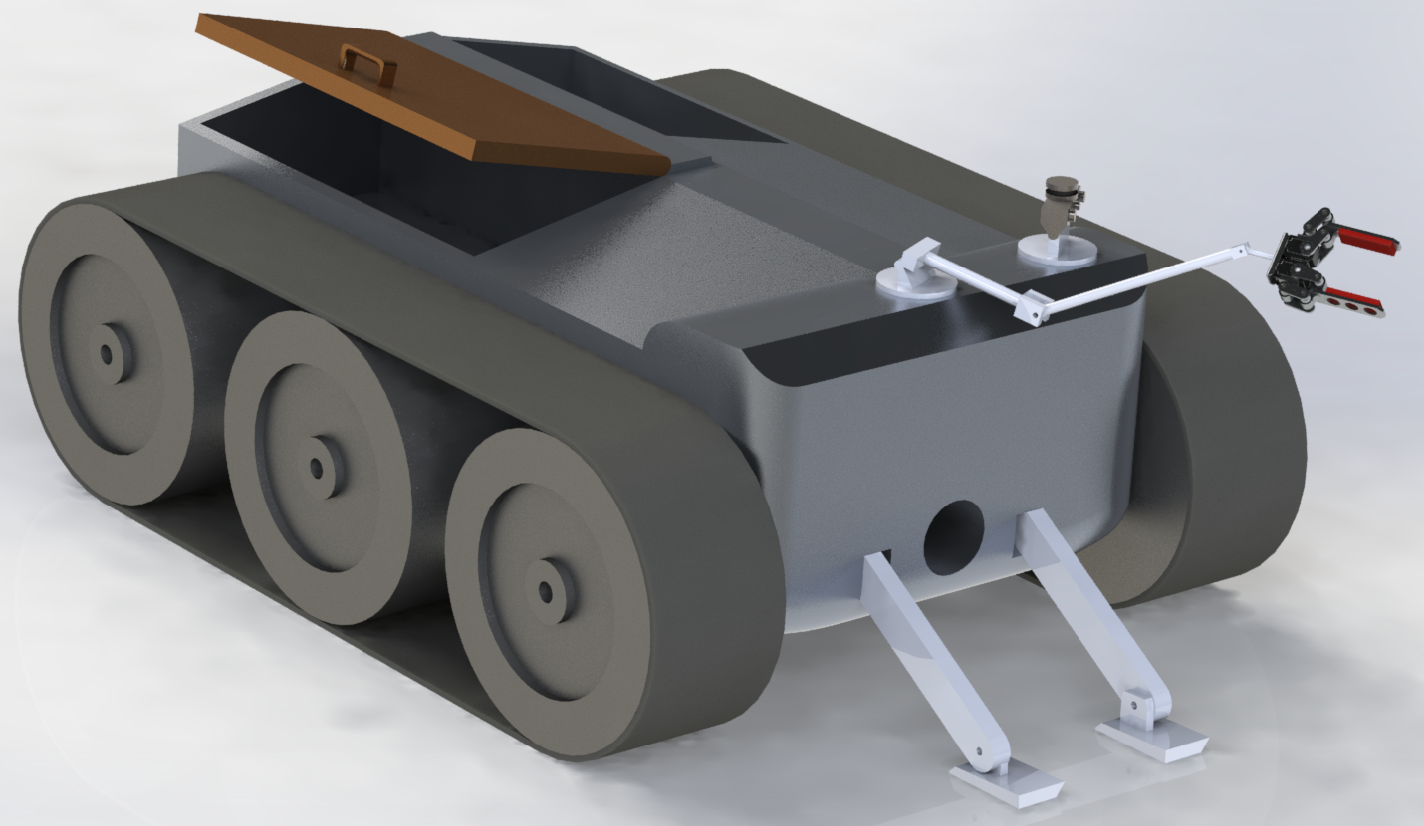
\includegraphics[width=1.0\linewidth]{Abbildungen/3D_model/prototype_front.png}}
  \caption{Kombinierter 3D Prototyp}
  \label{fig:model_proto}
\end{figure}
\section{Concept part}
From system level specification down to discipline specific documentation including diagrams and visualizations. Including a comprehensible derivation of your design decisions
\section{Evaluation}
(partly) implementation of system or (partly) Simulation of system e.g. in Matlab or microcontroller-based simulation of specific parts, or….

\section{Zusammenfassung und Ausblick\hfill\textnormal{\emph{Berger}}}
Zusammenfassend lässt sich sagen, dass alle Anforderungen aus Abschnitt \ref{sec:reqs} erfüllt wurden.
Eine genauere Darstellung, von welchen Implementierungen die einzelnen Anforderungen erfüllt werden,
lässt sich zusätzlich in der finalen Präsentation im GitHub Repository finden.
\footnote{https://github.com/BrunoBerger/Rescue-Robot/\linebreak
    blob/master/Präsentation/Final\_Presentation/\linebreak
    Final\_Project\_RescueRobot.pptx}
\\  

Als Weiterführung könnten weitere Tests mit dem 3D Modell durchgeführt werden,
um die Schwimmfähigkeit und die Effektivität des Propellers zu beweisen.
Erste flow-simulation in SolidWorks haben bereits einen recht schnellen Fluss
durch die Röhre des Roboters gezeigt.
Zusätzlich könnte die Stabilität des Greifers unter Last geprüft werden.

Auch das Design könnte in Zukunft noch verfeinert werden,
mit detaillierteren Hardware Schnittstellen 
und Protokollen für Randsituationen.

Die Software könnte noch um ein paar Features erweitert werden,
wie zum Beispiel diagonales Fahren des Roboters 
oder Sichteinschränkungen wie Nebel.

    


\section{Anhang}

\subsection{GitHub Übersicht\hfill\textnormal{\emph{Berger}}}

Zu Versionskontrolle wurde ein Git Repository genutzt 
das auf GitHub gehostet wird.
Darüber konnten wir gleichzeitig gemeinsam an dem Projekt arbeiten,
was auch in sehr gleichen Anteilen stattgefunden hat.
Die gesamte Arbeitszeit würden wir auf ungefähr 500 Stunden schätzen.

Zusätzlich wurden weitere Features von Github genutzt, 
wie die Project-Boards,
die als Erweiterung des Trello-Boards genutzt wurden 
um die Aufgaben für die jeweiligen Meilensteine festzuhalten.

Auch wurde GitHub-Actions genutzt 
um "Nightly Builds" von der Implementierung in C\# zu generieren.
Dabei wird das Projekt auf einer virtuellen Windows Installation gebaut 
und dann der Status des Builds dann in der Readme der Repositorys angezeigt.
Dies sieht aus wie in Abbildung \ref{fig:buildBadge}, 
falls der Build Vorgang nicht fehlschlägt
und Informiert schnell über den aktuellen Stand des Projekts.

\begin{figure}[H]
  \centering{
\includegraphics[width=0.3\linewidth]{Abbildungen/buildBadge.png}}
  \caption{Build Badge}
  \label{fig:buildBadge}
\end{figure}


\subsection{Source Code}

Der Quellcode für alle Implementierungen ist auf GitHub zu finden.
\footnote{https://github.com/BrunoBerger/Rescue-Robot/tree/master/Implementierung} % conference papers do not normally have an appendix

\section{Affidavit}
We (Bruno Berger, Lukas Walter, Melanie Löbel) herewith declare that we have composed the present paper and work ourself and without use of any other than the cited sources and aids. Sentences or parts of sentences quoted literally are marked as such; other references with regard to the statement and scope are indicated by full details of the publications concerned. The paper and work in the same or similar form has not been submitted to any examination body and has not been published. This paper was not yet, even in part, used in another examination or as a course performance.


\section{Conclusion}
The conclusion goes here.




% use section* for acknowledgment
\ifCLASSOPTIONcompsoc
  % The Computer Society usually uses the plural form
  \section*{Acknowledgments}
\else
  % regular IEEE prefers the singular form
  \section*{Acknowledgment}
\fi


The authors would like to thank...





% trigger a \newpage just before the given reference
% number - used to balance the columns on the last page
% adjust value as needed - may need to be readjusted if
% the document is modified later
%\IEEEtriggeratref{8}
% The "triggered" command can be changed if desired:
%\IEEEtriggercmd{\enlargethispage{-5in}}

% references section

\printbibliography


% that's all folks
\end{document}
